\documentclass{ecai2014}
\usepackage{times}
\usepackage{graphicx}
\usepackage{latexsym}

%%\ecaisubmission   % inserts page numbers. Use only for submission of paper.
                  % Do NOT use for camera-ready version of paper.

\begin{document}

\title{Guidelines for Preparing a Paper for the \\
European Conference on Artificial Intelligence}

\author{Name1 Surname1 \and Name2 Surname2 \and Name3 Surname3\institute{University of Leipzig,
Germany, email: somename@informatik.uni-leipzig.de} }

\maketitle
\bibliographystyle{ecai2014}

\begin{abstract}
  The purpose of this paper is to show a contributor the required
  style for a paper for ECAI-2014 and PAIS-2014. The specifications
  for layout are described so that non-\LaTeX\ users can create their
  own style sheet to achieve the same layout. The source for the
  sample file is available for \LaTeX\ users. The PostScript and the
  PDF file is available for all. A Microsoft Word template is also available.
 The layout is identical to ECAI'12
  papers. The publisher (IOS Press) will insert a footer for each
  page.
\end{abstract}

\section{PAGE LIMIT}
The page limit for ECAI-2014 and PAIS-2014 long papers is \textbf{6
  (six)} pages in the required format. The page limit for short
submissions is 2 pages. This is a strict limit. Overlength papers will
not be reviewed.

\section{GENERAL SPECIFICATIONS}
The following details should allow contributors to set up the general
page description for their paper:

\begin{enumerate}
\item The paper is set in two columns each 20.5 picas (86 mm) wide
  with a column separator of 1.5 picas (6 mm).

\item The typeface is Times Modern Roman.

\item The body text size is 9 point (3.15 mm) on a body of 11
point (3.85 mm) (i.e., 61 lines of text).

\item The effective text height for each page is 56 picas (237 mm).
The first page has less text height. It requires an additional footer
space of 3.5 picas (14.8 mm) for the copyright inserted by the publisher
and 1.5 picas (6 mm) of space before the title.
The effective text height of the first page is 51 picas (216 mm).

\item There are no running feet for the final camera-ready version of the
paper. The submission paper should have page numbers in the running feet.

\end {enumerate}

\section{TITLE, AUTHOR, AFFILIATION, COPYRIGHT
AND RUNNING FEET}
\subsection{Title}
The title is set in 20 point (7 mm) bold with leading of 22 point (7.7
mm), centered over the full text measure, with 1.5 picas (6 mm) of
space before and after.

\subsection{Author}
The author's name is set in 11 point (3.85 mm) bold with leading of 12
point (4.2 mm), centered over full text measure, with 1.5 picas (6 mm)
of space below. A footnote indicator is set in 11 point (3.85 mm)
medium and positioned as a superscript character.

\subsection{Affiliation}
The affiliation is set as a footnote to the first column. This is set
in 8 point (2.8 mm) medium with leading of 8.6 point (3.1 mm), with a
1 point (0.35 mm) footnote rule to column width.

\subsection{Copyright}
The copyright details will be inserted by the publisher.

\subsection{Running feet}
The running feet are inserted by the publisher. For submission you may
insert page numbers in the middle of the running feet. Do not,
however, insert page numbers for the camera-ready version of the
paper.

\section{ABSTRACT}
The abstract for the paper is set in 9 point (3.15 mm) medium, on a
body of 10 point (3.5 mm). The word Abstract is set in bold, followed
by a full point and a 0.5 pica space.

\section{HEADINGS}\label{heads}
Three heading levels have been specified:

\begin{enumerate}
\item{A level headings}

\begin{itemize}
\item The first level of heading is set is 11 point (3.85 mm) bold, on
  a body of 12 point (4.2 mm), 1.5 lines of space above and 0.5 lines
  of space below.

\item The heading is numbered to one digit with a 1 pica space
  separating it from the text.

\item The text is keyed in capitals and is unjustified.
\end{itemize}

\item{B level headings}
\begin{itemize}
\item The second level of heading is set is 11 point (3.85 mm) bold,
  on a body of 12 point (4.2 mm), 1.5 lines of space above and 0.5
  lines of space below.

\item The heading is numbered to two digits separated with a full
  point, with a 1 pica space separating it from the text.

\item The text is keyed in upper and lower case with an initial
  capital for first word only, and is unjustified.
\end{itemize}

\item{C level headings}
\begin{itemize}
\item The third level of heading is set is 10 point (3.5 mm) italic,
  on a body of 11 point (3.85 mm), 1.5 lines of space above and 0.5
  lines of space below.

\item The heading is numbered to three digits separated with a full
  point, with a 1 pica space separating it from the text.

\item The text is keyed in upper and lower case with an initial
  capital for first word only, and is unjustified.
\end{itemize}

\item{Acknowledgements}

  This heading is the same style as an A level heading but is not
  numbered.
\end{enumerate}

\section{TEXT}
The first paragraph of text following any heading is set to the
complete measure (i.e., do not indent the first line).

Subsequent paragraphs are set with the first line indented
by 1 pica (3.85 mm).

There isn't any inter-paragraph spacing.

\section{LISTS}
The list identifier may be an arabic number, a bullet, an em
rule or a roman numeral.

The items in a list are set in text size and indented by 1
pica (4.2 mm) from the left margin. Half a line of space is
set above and below the list to separate it from surrounding
text.

See layout of Section \ref{heads} on headings to see the results of the list macros.

\section{TABLES}
Tables are set in 8 point (2.8 mm) on a body of 10 point (3.5 mm).
The table caption is set centered at the start of the table, with
the word Table and the number in bold. The caption is set in medium
with a 1 pica (4.2 mm) space separating it from the table number.

A one line space separates the table from surrounding text.

\begin{table}
\begin{center}
{\caption{The table caption is centered on the table measure. If it
extends to two lines each is centered.}\label{table1}}
\begin{tabular}{lccccccc}
\hline
\rule{0pt}{12pt}
&\multicolumn{7}{c}{Processors}\\
&1&\multicolumn{3}{c}{2}&\multicolumn{3}{c}{4}\\
\cline{2-8}
\rule{0pt}{12pt}
Window&$\Diamond$&$\Diamond$&$\Box$&$\bigtriangleup$&$\Diamond$&$\Box$&$\bigtriangleup$
\\
\hline
\\[-6pt]
\quad1&1273&110&21.79&89\%&6717&22.42&61\%\\
\quad2&2145&116&10.99&50\%&5386&10.77&19\%\\
\quad3&3014&117&41.77&89\%&7783&42.31&58\%\\
\quad4&4753&151&71.55&77\%&7477&61.97&49\%\\
\quad5&5576&148&61.60&80\%&7551&91.80&45\%
\\
\hline
\\[-6pt]
\multicolumn{8}{l}{$\Diamond$ execution time in ticks\ \
$\Box$ speed-up values\ \
$\bigtriangleup$ efficiency values}
\end{tabular}
\end{center}
\end{table}

\section{FIGURES}
A figure caption is set centered in 8 point (2.8 mm) medium on a
leading of 10 point (3.5 mm).  It is set under the figure, with the
word Figure and the number in bold and with a 1 pica (4.2 mm) space
separating the caption text from the figure number.

One line of space separates the figure from the caption. A one line
space separates the figure from surrounding text.

\begin{figure}
\centerline{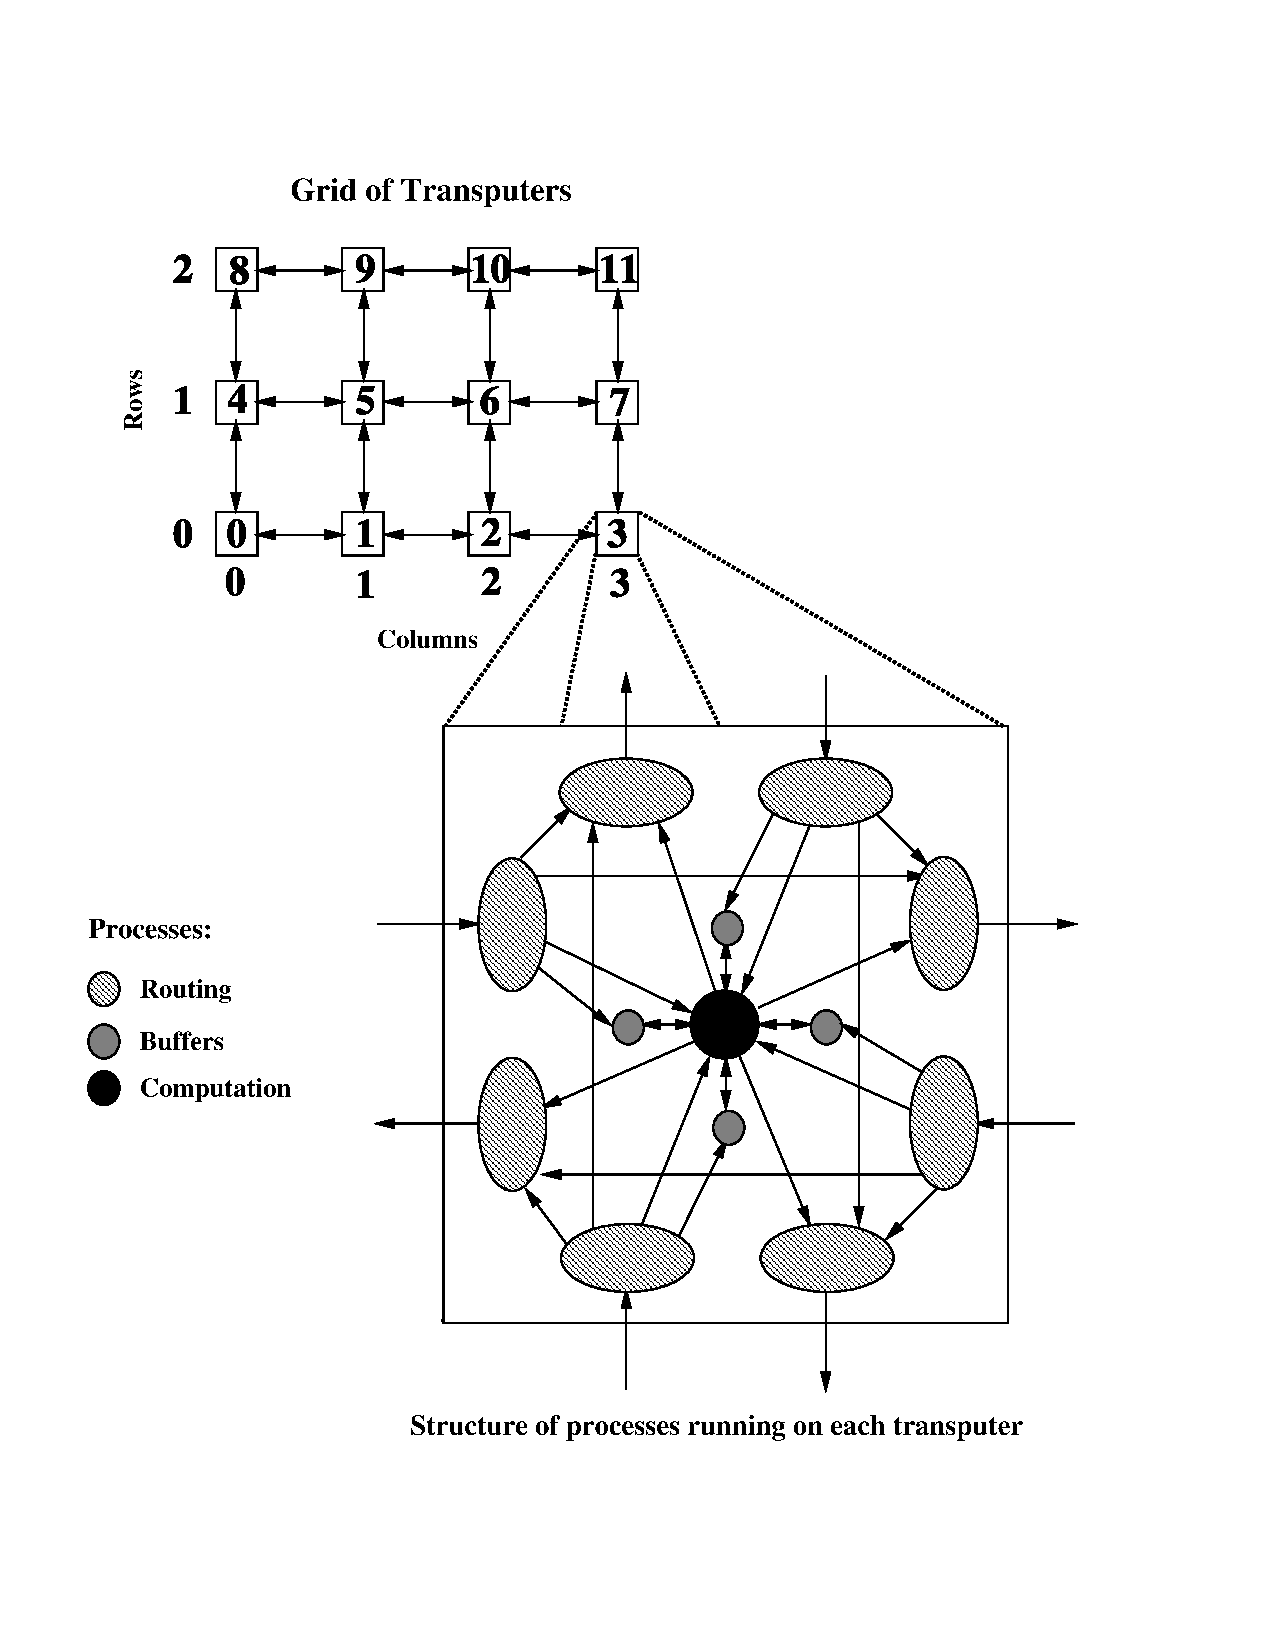
\includegraphics[height=3.5in]{ecaif01}}
\caption{Network of transputers and the structure of individual
processes } \label{procstructfig}
\end{figure}

\section{EQUATIONS}
A display equation is numbered, using arabic numbers in parentheses.
It is centered and set with one line of space above and below to
separate it from surrounding text. The following example is a simple
single line equation:

\begin{equation}
Ax=b
\label{thesystem}
\end{equation}

The next example is a multi-line equation:

\begin{eqnarray}
(x+y)(x-y) & = & x^2-xy+xy-y^2\\
(x+y)^2    & = & x^2+2xy+y^2
\end{eqnarray}

The equal signs are aligned in a multi-line equation.

\section{PROGRAM LISTINGS}
Program listings are set in 9 point (3.15 mm) Courier on a
leading of 11 point (3.85 mm). That is to say, a non-proportional
font is used to ensure the correct alignment.

A one line space separates the program listing from surrounding text.

\begin{verbatim}
void inc(x)
int* x;
{
    *x++;
}

int y = 1;
inc(&y);
printf("%d\n",y);
\end{verbatim}

\section{THEOREMS}
The text of a theorem is set in 9 point (3.15 mm) italic on a
leading of 11 point (3.85 mm). The word Theorem and its number
are set in 9 point (3.15 mm) bold.

A one line space separates the theorem from surrounding text.

\begin{theorem}
Let us assume this is a valid theorem. In reality it is a piece
of text set in the theorem environment.
\end{theorem}

\section{FOOTNOTES}
Footnotes are set in 8 point (2.8 mm) medium with leading of 8.6 point (3.1
mm), with a 1 point (0.35 mm) footnote rule to column
width\footnote{This is an example of a footnote that occurs in
the text. If the text runs to two lines the second line aligns
with the start of text in the first line.} .

\section{REFERENCES}
The reference identifier in the text is set as a sequential number in
square brackets. The reference entry itself is set in 8 point
(2.8 mm) with a leading of 10 point (3.5 mm), and appears
in the sequence in which it is cited in the paper.

\section{SAMPLE CODING}
The remainder of this paper contains examples of the specifications
detailed above and can be used for reference if required.

\section{PROGRAMMING MODEL}
\label{par}
Our algorithms were implemented using the \emph{single program,
  multiple data} model (SPMD). SPMD involves writing a single code
that will run on all the processors co-operating on a task. The data
are partitioned among the processors which know what portions of the
data they will work on \cite{kn:Golub89}.

\subsection{Structure of processes and processors}
\label{procstruct}
The grid has $P=P_{\rm{r}}\times P_{\rm{c}}$ processors, where
$P_{\rm{r}}$ is the number of rows of processors and $P_{\rm{c}}$ is
the number of columns of processors.

\subsubsection{Routing information on the grid}
\label{routing} A message may be either \emph{broadcast} or {\em
  specific}. A broadcast message originates on a processor and is
relayed through the network until it reaches all other processors. A
specific message is one that is directed to a particular target
processor.

Broadcast messages originate from a processor called \emph{central}
which is situated in the `middle' of the grid. This processor has
co-ordinates $(\lfloor P_{\rm{r}}/2 \rfloor,\lfloor P_{\rm{c}}/2
\rfloor)$.  Messages are broadcast using the \emph{row--column
  broadcast} algorithm (RCB), which uses the following strategy.  The
number of steps required to complete the RCB algorithm (i.e., until
all processors have received the broadcast value) is given by $\lfloor
P_{\rm{r}}/2\rfloor+\lfloor P_{\rm{c}}/2\rfloor$.

A specific message is routed through the processors using the
\emph{find-row--find-column} algorithm (FRFC) detailed in
\cite{kn:deCarlini91}.  The message is sent from the \emph{originator}
processor vertically until it reaches a processor sitting in the same
row as the \emph{target} processor. The message is then moved
horizontally across the processors in that row until it reaches the
target processor. An accumulation based on the recursive doubling
technique \cite[pp. 56--61]{kn:Modi88}, would require the same number
of steps as the RCB requires. If either the row or column of the
originator and target processors are the same then the message will
travel only in a horizontal or vertical direction, respectively (see
\cite{kn:Smith85}).

\section{DATA PARTITIONING}
\label{datapart}
We use \emph{data partitioning by contiguity}, defined in the
following way. To partition the data (i.e., vectors and matrices)
among the processors, we divide the set of variables
\mbox{$V=\{\,i\,\}_{i=1}^{N}$} into $P$ subsets
$\{\,W_{p}\,\}_{p=1}^{P}$ of $s=N/P$ elements each. We assume without
loss of generality that $N$ is an integer multiple of $P$. We define
each subset as $W_{p}=\{(p-1)s+j\}_{j=1}^{s}$ (see
\cite{kn:Schofield89}, \cite{kn:daCunha92a} and \cite{kn:Atkin} for
details).

Each processor $p$ is responsible for performing the computations over
the variables contained in $W_{p}$. In the case of vector operations,
each processor will hold segments of $s$ variables. The data
partitioning for operations involving matrices is discussed in Section
\ref{mv}.
\section{LINEAR ALGEBRA OPERATIONS}
\label{blas}
\subsection{Saxpy}
\label{saxpy}
The saxpy $w=u+\alpha v$ operation, where $u$, $v$ and $w$ are vectors
and $\alpha$ is a scalar value, has the characteristic that its
computation is \emph{disjoint elementwise} with respect to $u, v$ and
$w$. This means that we can compute a saxpy without any communication
between processors; the resulting vector $w$ does not need to be
distributed among the processors. Parallelism is exploited in the
saxpy by the fact that $P$ processors will compute the same operation
with a substantially smaller amount of data. The saxpy is computed as
\begin{equation}
w_{i}=u_{i}+\alpha v_{i},\quad \forall i\in\{W_{p}\}_{p=1}^{P}
\label{distsaxpy}
\end{equation}
\subsection{Inner-product and vector 2-norm}
\label{utv}
The inner-product $\alpha=u^{T}v=\sum_{i=1}^{N}{u_{i}v_{i}}$ is an
operation that involves accumulation of data, implying a high level of
communication between all processors. The mesh topology and the
processes architecture used allowed a more efficient use of the
processors than, for instance, a ring topology, reducing the time that
processors are idle waiting for the computed inner-product value to
arrive, but the problem still remains. The use of the SPMD paradigm
also implies the global broadcast of the final computed value to all
processors.

The inner-product is computed in three distinct phases. Phase 1 is the
computation of partial sums of the form
\begin{equation}
\alpha_{p}=\sum_{\forall i\in\{W_{p}\}}{u_{i}\times v_{i}},\quad p=1,\ldots,P
\label{distutv}
\end{equation}

The accumulation phase of the inner-product using the RCA algorithm is
completed in the same number of steps as the RCB algorithm (Section
\ref{routing}). This is because of the need to relay partial values
between processors without any accumulation taking place, owing to the
connectivity of the grid topology.

The vector 2-norm $\alpha=||\,u\,||_{2}=\sqrt{u^{T}u}$ is computed
using the inner-product algorithm described above. Once the
inner-product value is received by a processor during the final
broadcast phase, it computes the square root of that value giving the
required 2-norm value.

\subsection{Matrix--vector product}
\label{mv}
For the matrix--vector product $v=Au$, we use a \emph{column
  partitioning} of $A$.  Each processor holds a set $W_{p}$ (see
Section \ref{datapart}) of $s$ columns each of $N$ elements of $A$ and
$s$ elements of $u$.  The $s$ elements of $u$ stored locally have a
one-to-one correspondence to the $s$ columns of $A$ (e.g. a processor
holding element $u_{j}$ also holds the $j$-th column of $A$). Note
that whereas we have $A$ partitioned by columns among the processors,
the matrix--vector product is to be computed by \emph{rows}.

The algorithm for computing the matrix--vector product using column
partitioning is a generalization of the inner-product algorithm
described in Section \ref{utv} (without the need for a final broadcast
phase). At a given time during the execution of the algorithm, each
one of $P-1$ processors is computing a vector $w$ of $s$ elements
containing partial sums required for the segment of the vector $v$ in
the remaining `target' processor.  After this computation is complete,
each of the $P$ processors stores a vector $w$.  The resulting segment
of the matrix--vector product vector which is to be stored in the
target processor is obtained by summing together the $P$ vectors $w$,
as described below.

Each processor other than the target processor sends its $w$ vector to
one of its neighboring processors. A processor decides whether to send
the vector in either the row or column direction to reach the target
processor based on the FRFC algorithm (see Section \ref{routing}). If
a vector passes through further processors in its route to the target
processor the $w$ vectors are accumulated. Thus the target processor
will receive at most four $w$ vectors which, when summed to its own
$w$ vector, yield the desired set of $s$ elements of $v$.

\subsection{Matrix--vector product---finite-difference approximation}
We now consider a preconditioned version of the conjugate-gradients
method \cite{kn:Golub89}. Note that we do not need to form $A$
explicitly.  This implies a very low degree of information exchange
between the processors which can be effectively exploited with
transputers, since the required values of $u$ can be exchanged
independently through each link.

The preconditioning used in our implementations is the polynomial
preconditioning (see \cite{kn:Saad85}, \cite{kn:Eisenstat81},
\cite{kn:Adams85} and \cite{kn:Johnson83}), which can be implemented
very efficiently in a parallel architecture since it is expressed as a
sequence of saxpys and matrix--vector products.

We have $l$ rows and columns in the discretization grid, which we want
to partition among a $P_{\rm{r}}\times P_{\rm{c}}$ mesh of
processors. Each processor will then carry out the computations
associated with a block of $\lfloor
l/P_{\rm{r}}\rfloor+\hbox{sign}\left( l\bmod P_{\rm{r}}\right)$ rows
and $\lfloor l/P_{\rm{c}}\rfloor+\hbox{sign}\left( l\bmod
  P_{\rm{c}}\right)$ columns of the interior points of the grid.

The matrix--vector product using the column partitioning is highly
parallel. Since there is no broadcast operation involved, as soon as a
processor on the boundary of the grid (either rows or columns) has
computed and sent a $w_{p}$ vector destined to a processor `A', it can
compute and (possibly) send a $w_{p}$ vector to processor `B', at
which time its neighboring processors may also have started computing
and sending their own $w$ vectors to processor `B'.

At a given point in the matrix--vector product computation, the
processors are computing $w$ vectors destined to processor A. When
these vectors have been accumulated in the row of that processor (step
1), the processors in the top and bottom rows compute and send the $w$
vectors for processor B, while the processors on the left and right
columns of the row of processor A send the accumulated $r$ vectors to
processor A (step 2). Processor A now stores its set of the resulting
$v$ vector (which is the accumulation of the $w$ vectors). In step 3,
the processors in the bottom row compute and send the $w$ vectors for
processor C while the processor at the left-hand end of the row of
processor B sends the accumulated $w$ vectors of that column towards
processor B. The next steps are similar to the above.

In our implementation, we exploit the geometry associated with the
regular grid of points used to approximate the PDE. A geometric
partitioning is used to match the topology and connectivity present in
the grid of transputers (Section \ref{procstruct}).

The discretization of the PDE is obtained by specifying a grid size
$l$ defining an associated grid of $N=l^2$ interior points (note that
this is the order of the linear system to be solved). With each
interior point, we associate a set of values, namely the coefficients
$C, N, S, E\,$ and $W$.

\section{CONCLUSION}
We have shown that an iterative method such as the preconditioned
conjugate-gradients method may be successfully parallelized by using
highly efficient parallel implementations of the linear algebra
operations involved. We have used the same approach to parallelize
other iterative methods with similar degrees of efficiency (see
\cite{kn:daCunha92a} and \cite {kn:daCunha92b}).

\ack We would like to thank the referees for their comments, which
helped improve this paper considerably

\bibliography{ecai2014}
\end{document}
%%%%%%%%%%%%%%%%%%%%%%%%%%%%%%%%%%%%%%%%%%%%%%%%%%%%%%%%%%%%%%%%%%%%%%
